\documentclass{article}
\usepackage[utf8]{inputenc}
\usepackage[T1]{fontenc}
\usepackage{xcolor}
\usepackage{tikz}
\usetikzlibrary{positioning, shapes.geometric, arrows}
\usetikzlibrary{positioning,calc,bayesnet,external}
\usepackage{pgfplots}
\usepackage{amsmath}

\begin{document}

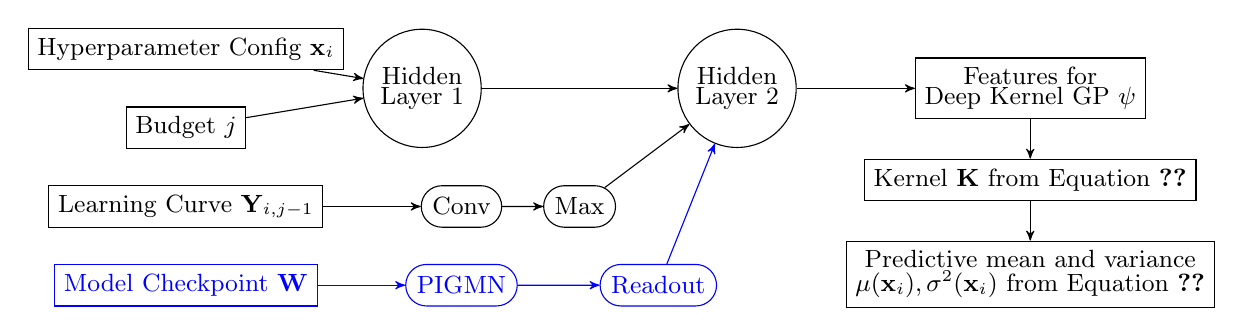
\begin{tikzpicture}[
  node distance=1.5cm,
  >=stealth',
  every node/.style={align=center, font=\fontsize{9}{0}\selectfont},
]

\tikzstyle{boxstyle}=[rectangle,draw=black,minimum size=15]
\tikzstyle{circlestyle}=[circle,draw=black,minimum size=15]
\tikzstyle{roundedrect}=[rounded rectangle,draw=black,minimum size=15]
\tikzstyle{blueroundedrect}=[rounded rectangle,draw=blue,minimum size=15]
\tikzstyle{bluerectangle}=[rectangle,draw=blue,minimum size=15]
\tikzstyle{bluearrow}=[->, draw=blue]

\node[boxstyle](x_input) at (0, 2) {Hyperparameter Config $\textbf{x}_{i}$};
\node[boxstyle](b_input) at (0, 1) {Budget $j$};
\node[boxstyle](lc_input) at (0, 0) {Learning Curve $\mathbf{Y}_{i,j-1}$};
\node[bluerectangle](pigm_input) at (0, -1) {\textcolor{blue}{Model Checkpoint $\mathbf{W}$}};


\node[circlestyle](layer1) at (3, 1.5) {Hidden\\Layer 1};
\node[circlestyle](layer2) at (7, 1.5) {Hidden\\Layer 2}; 

\node[roundedrect](conv) at (3.5, 0) {Conv}; 
\node[roundedrect](max) at (5, 0) {Max}; 
\node[blueroundedrect](pigm) at (3.5, -1) {\textcolor{blue}{PIGMN}};
\node[blueroundedrect](readout) at (6, -1) {\textcolor{blue}{Readout}};

\draw[->] (x_input) -- (layer1);
\draw[->] (b_input) -- (layer1);
\draw[->] (lc_input) -- (conv);
\draw[bluearrow] (pigm_input) -- (pigm);
\draw[->] (layer1) -- (layer2);
\draw[->] (conv) -- (max);
\draw[->] (max) -- (layer2);
\draw[bluearrow] (pigm) -- (readout);
\draw[bluearrow] (readout) -- (layer2);


\node[boxstyle, right=of layer2] (output) {Features for\\Deep Kernel GP $\psi$};
\draw[->] (layer2) -- (output);

\node[boxstyle, below=of output, yshift=1cm] (kernelOutput) {Kernel $\mathbf{K}$ from Equation~\ref{eq:weight_kernel}};
\draw[->] (output) -- (kernelOutput);

\node[boxstyle, below=of kernelOutput, yshift=1cm] (mean_var_Output) {Predictive mean and variance\\ $\mu(\mathbf{x}_{i}), \sigma^2(\mathbf{x}_{i})$ from Equation~\ref{eq:pred_mean_var}};
\draw[->] (kernelOutput) -- (mean_var_Output);

\end{tikzpicture}

\end{document}